\documentclass[a4paper, 11pt]{article}
\usepackage{graphicx}
\usepackage[frenchb]{babel}
\usepackage[utf8]{inputenc}
\title{Rapport du projet SGBD - Foyer}
\author{Boisson Pacien - Sarlin Nicolas - Taton Sven}
\date{Vendredi 14 Décembre 2012} 

%Début du rapport
\begin{document}
\maketitle
\tableofcontents
\newpage
\section{Introduction}
Le projet consiste à réaliser une base de données contenant les informations nécéssaires à l'organisation d'un foyer étudiant.\\
Le foyer étudiant organise des évènements pour les élèves, au cours desquels ces derniers utilisent des jeux, il serait utile de conserver un historique des évènements organisés et des jeux utilisés pour l'occasion. Le foyer est aussi une bibliothèque associative, les élèves pouvant y emprunter des livres, il serait donc aussi utile de conserver un historique des emprunts de livres.
\newpage
\part{Modélisation des données}
\setcounter{section}{0}
\section{Description du contexte de l'application}
Tous les élèves de l'école sont des utilisateurs du foyer, chaque élève est caractérisé par l'année à laquelle il quittera l'école, sa promo. Parmi ces élèves, certains sont ou ont été membres du bureau, donc administrateurs du foyer pendant une année. Le foyer organise des évènements ponctuels dans divers lieux, au cours desquels il utilise un ou plusieurs jeux, et auxquels les élèves peuvent participer. Un livre donné est disponible en un ou plusieurs exemplaires au foyer, ces livres peuvent être empruntés par les élèves.
\section{Modèle entité-association}
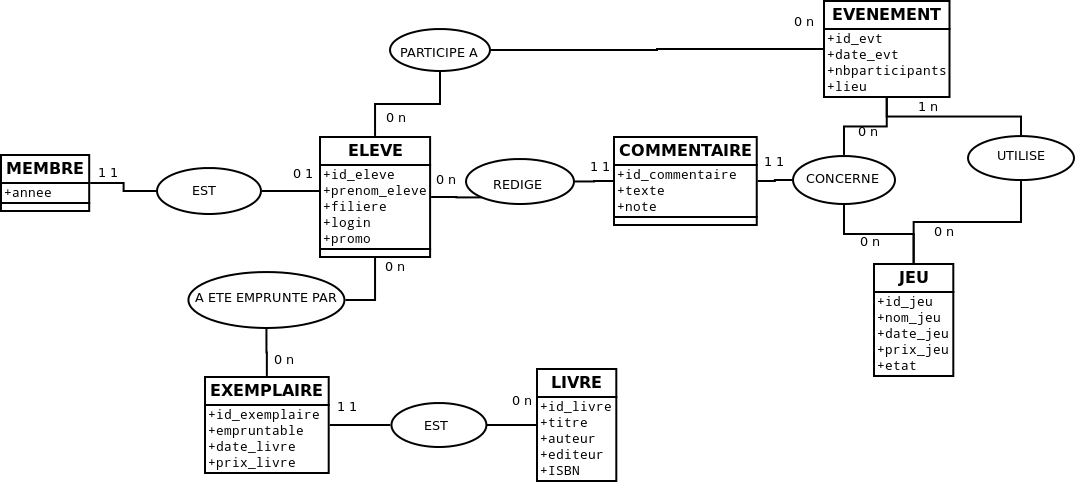
\includegraphics[width=1.2\textwidth]{ER.png}
Les conventions de nommage utilisées sont les suivantes : Les noms d'entité/association sont écrits en majuscule. Les clés sont en minuscule. En cas d'ambigu\"ité entre deux noms, on rajoute un symbole \_, suivi du nom de la table en minuscule. Les clés primaires commencent par id.
\paragraph{}
Les entités sont celles demandées dans le sujet, à l'exception de l'entité EXEMPLAIRE. Celle ci a été créée pour distinguer le livre au sens virtuel (qui possède titre, auteur, editeur et ISBN) de l'objet physique. Ainsi, un élève emprunte un exemplaire et non pas un livre. Nous avons aussi choisi de réaliser une association A ETE EMPRUNTE PAR (emprunts actuels et passés plut\^ot que EST EMPRUNTE PAR afin de pouvoir conserver l'historique des emprunts (utile pour les requ\^etes de statistiques).\\
Nous considérons aussi que lorsque le sujet mentionne l'action pour un élève de lire un livre, il s'agit en fait de l'emprunter (on n'enregistre pas dans la base de donnée à chaque fois qu'un élève consulte un livre sur place). 
\section{Liste des opérations prévues sur la base}

\subsection{Opérations sur les élèves}
\begin{itemize}
\item Obtenir la liste des èleves de l'école.
\item Obtenir l'historique des élèves de l'école.
\item Obtenir les informations (nom, prénom, promo, login) d'un élève donné.
\item Ajouter, modifier, supprimer un élève à la liste.
\end{itemize}
\subsection{Opérations sur les membres du bureau}
\begin{itemize}
\item Obtenir un historique complet des membres du bureau, ou obtenir la liste des membres du bureau pendant une année donnée.
\item Obtenir la liste des membres du bureau qui ont participé à un évènement après avoir effectué leur mandat.
\end{itemize}
\subsection{Opérations sur les évènements}
\begin{itemize}
\item Ajouter, modifier, supprimer un évènement.
\item Obtenir la liste des évènements auquels un membre va participer.
\item Obtenir la liste des jeux utilisés pour un évènement.
\item Obtenir le nombre de participants à un évènement donné.
\item Afficher tous commentaires écrits pour un évènement.
\end{itemize}
\subsection{Opérations sur les livres}
\begin{itemize}
\item Ajouter, modifier, supprimer un livre.
\item Obtenir l'historique des emprunts d'un livre.
\item Obtenir la liste et l'etat des exemplaires d'un livre.
\item Obtenir la liste des livres actuellement empruntés et disponibles à l'emprunt.
\item Obtenir la moyenne des emprunts de livre sur une année.
\item Obtenir le classement des livres les plus lus.
\item Afficher les commentaires écrits sur un livre.
\end{itemize}
\subsection{Opérations sur les jeux}
\begin{itemize}
\item Ajouter, modifier, supprimer un jeu.
\item Obtenir un classement des jeux selon leur utilisation lors des évènements.
\item Afficher les commentaires écrits sur un jeu.
\end{itemize}

\newpage
\part{Schéma relationnel}
\setcounter{section}{0}
\section{Passage au relationnel}
Le passage au modèle relationnel nécessite d'étudier les particularités de chaque association pour créer les bonnes relations. Certaines nécessitent la création de nouvelles tables, d'autres se contentent d'un ajout de clé étrangère.
\section{Contraintes d'intégrité et dépendances fonctionnelles}
\section{Schéma relationnel en $3^{eme}$ forme normale}
\section{Création de vues}
Afin de faciliter certaines actions et réduire les requêtes SQL, nous avons également créé des vues concernant l'historique des membres, et les livres en cours d'emprunt.

\newpage
\part{Implantation}
\setcounter{section}{0}
\section{Création de la base de données}
Nous avons choisit d'utiliser une base de données de type MySQL, correspondant au mieux a notre interface, et proposant des fonctionnalités telles que l'auto incrementations assez utiles.
\section{Implémentation des commandes SQL}
\subsection{Opérations sur les membres du bureau}
\paragraph{}
Historique complet des membres du bureau, ou liste des membres du bureau pendant une année donnée.
\begin{verbatim}
SELECT *
FROM ELEVE, MEMBRE
WHERE ELEVE.id_eleve = MEMBRE.id_eleve AND MEMBRE.annee < YEAR(NOW());
\end{verbatim}
\paragraph{}
Liste des membres du bureau qui ont participé à un évènement après avoir effectué leur mandat.
\begin{verbatim}
SELECT DISTINCT *
FROM ELEVE, EVENEMENT, PARTICIPE, MEMBRE
WHERE ELEVE.id_eleve = PARTICIPE.id_eleve
AND ELEVE.id_eleve = MEMBRE.id_eleve
AND PARTICIPE.id_evt = EVENEMENT.id_evt
AND YEAR(EVENEMENT.date_evt) > MEMBRE.annee;
\end{verbatim}
\subsection{Opérations sur les élèves}
\paragraph{}
Informations (nom, prénom, promo, login) d'un élève donné.
\begin{verbatim}
SELECT *
FROM ELEVE;
\end{verbatim}
\paragraph{}
Commentaires écrits par l'élève à propos d'un jeu ou d'un livre.
\begin{verbatim}
SELECT IFNULL(texte, 'Non renseigné') AS texte,
       IFNULL(note, 'Non renseigné') AS note,
       IF(COMMENTAIRE.id_evt, 'evt', 'jeu') AS type, 
       IF(COMMENTAIRE.id_evt, COMMENTAIRE.id_evt, COMMENTAIRE.id_jeu) AS id
FROM COMMENTAIRE
WHERE id_eleve = 1;
\end{verbatim}
\subsection{Opérations sur les évènements}
\paragraph{}
Liste des évènements auquels a participé un membre pendant une année donnée.
\begin{verbatim}
SELECT *
FROM EVENEMENT, PARTICIPE
WHERE PARTICIPE.id_eleve = 18
AND PARTICIPE.id_evt = EVENEMENT.id_evt
AND year(EVENEMENT.date_evt) = YEAR(NOW())
\end{verbatim}
\paragraph{}
Nombre de participants à un évènement donné.
\begin{verbatim}
SELECT COUNT(*)
FROM EVENEMENT, PARTICIPE
WHERE EVENEMENT.id_evt = PARTICIPE.id_evt
AND EVENEMENT.id_evt = 3;
\end{verbatim}
\paragraph{}
Commentaires écrits sur un évènement.
\begin{verbatim}
SELECT texte, note 
FROM COMMENTAIRE
WHERE COMMENTAIRE.id_evt = 4;
\end{verbatim}
\subsection{Opérations sur les livres}
\paragraph{}
Liste des emprunts par élève pour un livre donné.
\begin{verbatim}
SELECT date_rendu, nom_eleve  
FROM ELEVE, LIVRE, EXEMPLAIRE, EMPRUNT  
WHERE ELEVE.id_eleve = EMPRUNT.id_eleve  
AND EMPRUNT.id_exemplaire = EXEMPLAIRE.id_exemplaire  
AND EXEMPLAIRE.id_livre = LIVRE.id_livre  
AND LIVRE.titre = "Fascination" 
ORDER BY date_rendu DESC;
\end{verbatim}
\paragraph{}
Moyenne des emprunts de livre sur une année donnée.
\begin{verbatim}
// Ici pour l'année 2012
SELECT sum(total.an)/ 12 AS moyenne 
FROM (SELECT count(*) AS an 
    FROM EMPRUNT 
    WHERE YEAR(date_rendu)='2012' 
    GROUP BY MONTH(date_rendu)) AS total;
\end{verbatim}
\paragraph{}
Classement des livres les plus lus.
\begin{verbatim}
SELECT LIVRE.titre, count(*) as nombre 
FROM LIVRE, EXEMPLAIRE, EMPRUNT 
WHERE LIVRE.id_livre = EXEMPLAIRE.id_livre 
AND EXEMPLAIRE.id_exemplaire = EMPRUNT.id_exemplaire 
GROUP BY LIVRE.titre 
ORDER BY nombre DESC;
\end{verbatim}
\subsection{Opérations sur les jeux}
\paragraph{}
Liste des jeux utilisés pour un évènement donné.
\begin{verbatim}
// Ici avec l'évènement d'ID 3
SELECT *
FROM JEU, EVENEMENT, UTILISE
WHERE JEU.id_jeu = UTILISE.id_jeu
AND UTILISE.id_evt = EVENEMENT.id_evt
AND EVENEMENT.id_evt = 3;
\end{verbatim}
\paragraph{}
Classement des jeux selon leur utilisation lors des évènements.
\begin{verbatim}
SELECT nom_jeu, SUM(nombre) AS total
FROM JEU, UTILISE, 
     (SELECT EVENEMENT.id_evt, count(*) AS nombre 
     FROM PARTICIPE, EVENEMENT 
     WHERE EVENEMENT.id_evt = PARTICIPE.id_evt 
     GROUP BY EVENEMENT.id_evt) AS PARTICIPATION
WHERE JEU.id_jeu = UTILISE.id_jeu
AND UTILISE.id_evt = PARTICIPATION.id_evt
GROUP BY JEU.id_jeu
ORDER BY total DESC;
\end{verbatim}
\paragraph{}
Commentaires écrits sur un jeu.
\begin{verbatim}
// Ici pour le jeu d'ID 4
SELECT texte, note 
FROM COMMENTAIRE
WHERE COMMENTAIRE.id_jeu = 4;
\end{verbatim}
\section{Problèmes rencontrés}
\subsection{Suppression de clés étrangères}
Nous avons été confronté a un probleme lors de la suppression de certaines informations. Par exemple, lors de la suppression d'un élève, la base de données refusait de supprimer la ligne correspondante dans ELEVE car il restait des lignes contenant les memes clés dans les tables MEMBRE, EMPRUNT et PARTICIPE. Ce problème a été résolu en ajoutant la fonctionalité CASCADE lors de la création de la base de données. Nous avons donc ajouté ces lignes dans les tables contenant des clés étrangères (exemple avec MEMBRE ici) :
\begin{verbatim}
  INDEX `fk_Membres_Eleves` (`id_eleve` ASC) ,
  CONSTRAINT `fk_Membres_Eleves`
    FOREIGN KEY (`id_eleve` )
    REFERENCES `projetSGBD`.`ELEVE` (`id_eleve` )
    ON DELETE CASCADE)  // Supprime la ligne correspondante dans MEMBRE lors de la suppression dans ELEVE
\end{verbatim}
\subsection{Dernier element inseré}
Lors de l'ajout de certaines informations, il est parfois necessaire de faire des insertions dans plusieurs tables differentes. Or, nous avons, pour les tables possedant des index, utilisé la fonctionnalité AUTO_INCREMENT de MySQL, qui permet d'inserer automatiquement un index unique aux données. 
\\Le problème rencontré, est, par exemple, lors de l'ajout d'un membre. Il faut faire une insertion dans ELEVE puis dans MEMBRE. Cependant, dans MEMBRE, il faut indiquer l'index de l'eleve ajouté, ce que nous ne connaissons pas, car nous ne l'avons pas definit nous même. Pour cela MySQL nous propose une fonction, nommée $LAST_INSERT_ID()$ retournant le dernier index primaire créé automatiquement. Ainsi, nous pouvons creer la ligne dans MEMBRE selon le dernier ajout dans ELEVE. Nous avons verifié qu'il n'y a pas de probleme d'asynchronisme, car cette fonction est dependante de la session en cours, donc si plusieurs ajouts se font simultanement, il n'y a pas risque de chevauchement.

\newpage
\part{Utilisation}
\setcounter{section}{0}
\section{Description de l'environnement d'exécution}
La creation d'un modele de donnée solide est important pour la mise en oeuvre d'un tel projet. Mais elle n'a d'interet que si l'on fournit à l'utilisateur une interface pratique d'utilisation. Celle-ci doit simplifier l'acces, la visibilité, l'ajout et la modification de données tout en respectant la structure de données.
\\Pour ce projet nous avons choisit de construire une interface web, car c'est une des solutions les plus pratiques pour créer une interface utilisateur agréable rapidement. Nous avons donc créé un site web dynamique avec PHP, modulaire, dans lequel il est rapide d'ajouter des nouvelles fonctionnalités grâce au coté objet de PHP. En effet, chaque page est un objet héritant d'une page de base possedant les fonctionnalités necessaires pour les actions realisées (design, accès base de donnée simplifiée, configuration globale, outils divers). 
\\Afin que d'avoir une experience utilisateur plus agréable, nous nous sommes servis de la librairie jQuery permettant d'avoir des pages soignées et dynamiques, notament grace aux widget et l'utilisation d'AJAX. 
\section{Notice d'utilisation}
\subsection{Logiciels necessaires}
Nous avons conçu ce site web grâce a la combinaison PHP5/MySQL.
Le site a été testé et est fonctionnel avec les logiciels suivants :
\begin{itemize}
\item Apache 2
\item PHP 5.4 avec mysqli activé
\item MySQL 5.5
\item Chromium 22 / Firefox 16 avec javascript activé
\end{itemize}
\subsection{Première utilisation}
Vous devez placer tous les fichiers du site dans votre dossier d'hebergement. La première chose a faire est d'ouvrir le fichier à la racine nommé $config.php$. Il contient les informations de bases pour se connecter a la base de donnée. Veuillez modifier les variables $\$config->mysqlDB$ adéquates pour fonctionner sur votre serveur MySQL. 
Vous pouvez alors accéder avec votre navigateur au site.
\\ \textit{Note : 
En fonction de la configuration de MySQL, il sera peut-etre necessaire de créer au préalable la base de données indiquée dans ce fichier. Dans ce cas, une fois la base de données créée, aller dans le site puis dans \textbf{Outils} enfin \textbf{Reinitialiser la base de donnees}.}
\section{Description des interfaces éventuelles}
\subsection{Fonctionnement du site}
Les differents accès aux informations sont regroupées par categories, les livres, les jeux, les evenements et les élèves. Pour chacune de celles ci, la liste est affichée, avec possiblité d'ajouter un élement, et pour chaque élement, on peut editer, supprimer ou d'obtenir plus d'information sur cet élement en particulier.
\\Les actions concernant un élève en particulier n'est possible que si cet élève est connecté. Pour ceci, consulter la liste des élèves, noter les login et les utiliser dans "Se connecter". Il est alors possible d'emprunter un livre, de s'inscrire a un évènement ou faire un commentaire. Les résultats de ces actions sont visibles dans les categories correspondantes.
\\Il est possible d'éxecuter directement une requète SQL dans le site, afin de pouvoir effectuer ses propres tests. Ceci ne serait pas mis a disposition si le site etait vraiment deployé, pour des raisons de securité.
\subsection{Ce qu'il manque à l'interface}
Beaucoup de fonctionnalités auraient pu être rajoutées mais cela n'a pas été effectué car n'etant pas demandé dans le sujet et ayant peu de rapport avec les bases de données, auraient eu peu d'interêt ici. Cependant, en pratique, certaines pourraient être indispensable, a savoir :
\begin{itemize}
\item Connexion par mot de passe pour les élèves. 
\item Modification des données uniquement par les membres actuels du bureau. A savoir ajout d'évènement, de membres, de livres, de jeux et modification de ceux-ci.
\item Meilleure gestion des exemplaires des livres. Il n'est actuellement pas possible d'ajouter un exemplaire a un livre.
\end{itemize}

\end{document}
